\section{The Proposal}


In summary, our two primary goals in order to improve perfor- mance/energy efficiency are:
• Reducing coherence misses
• Reducing the amount of coherence traffic
In the case of computing with approximable data, we can allow the usage of data that does not necessarily have the latest value. This would enable us to (i) drop writebacks and invalidates to memory and other cores during processor writes and (ii) execute on imprecise stale data in the case of a processor read.
Ignoring all coherence messages for shared data would lead to a highly approximate and imprecise system. We, however, need to limit this imprecision by enabling coherence messages in such a manner so as to obtain an acceptable trade-off between precision and performance.

In this section, we describe our proposed approximate protocol. The key observation behind our proposed idea is that all updates are not equal. In fact, some writes make a huge difference while other slightly modify the previous data. As a result, we could treat them differently. It means that when there are only a small updates to the cache line, we might be able to avoid propagating those writes to other threads and eliminate the coherence messages plus avoid potential coherence misses.

The coherence traffic and coherence misses are mainly generated from transitions to the "Modified" state which results in invalidations to the same cachelines in other caches. In order to minimize these transi- tions, we propose to add another state to the cache coherence protocol to track modified data - "Highly Modified (H)" state. This state is treated in the same manner as a real modified state, where invalidates are sent to the directory and other caches and writebacks to DRAM are generated. The other modified state "Modified (M)" does not cause invalidations to data in the directory or other caches. In this case it is possible for a cacheline to exist simultaneously in the shared (S) and modified (M) states. The modified state primarily exists to control the transition from "H" and "M" and control impreci- sion. Upon eviction of data from the cache, data in the "M" state is still written back to memory as usual.

Figure 5 shows our proposed approximate cache coherence protocol. As it is shown in figure 5, when a big update reaches cache controller, it is treated as a regular write. It means that the cache line makes a transition to the H state and invalidate all other copies. Those copies could be in modified, shared or exclusive state. When a small updates gets to the cache controller, it simply makes a transition to the modified state.  



\begin{figure}[h]
  \centering
  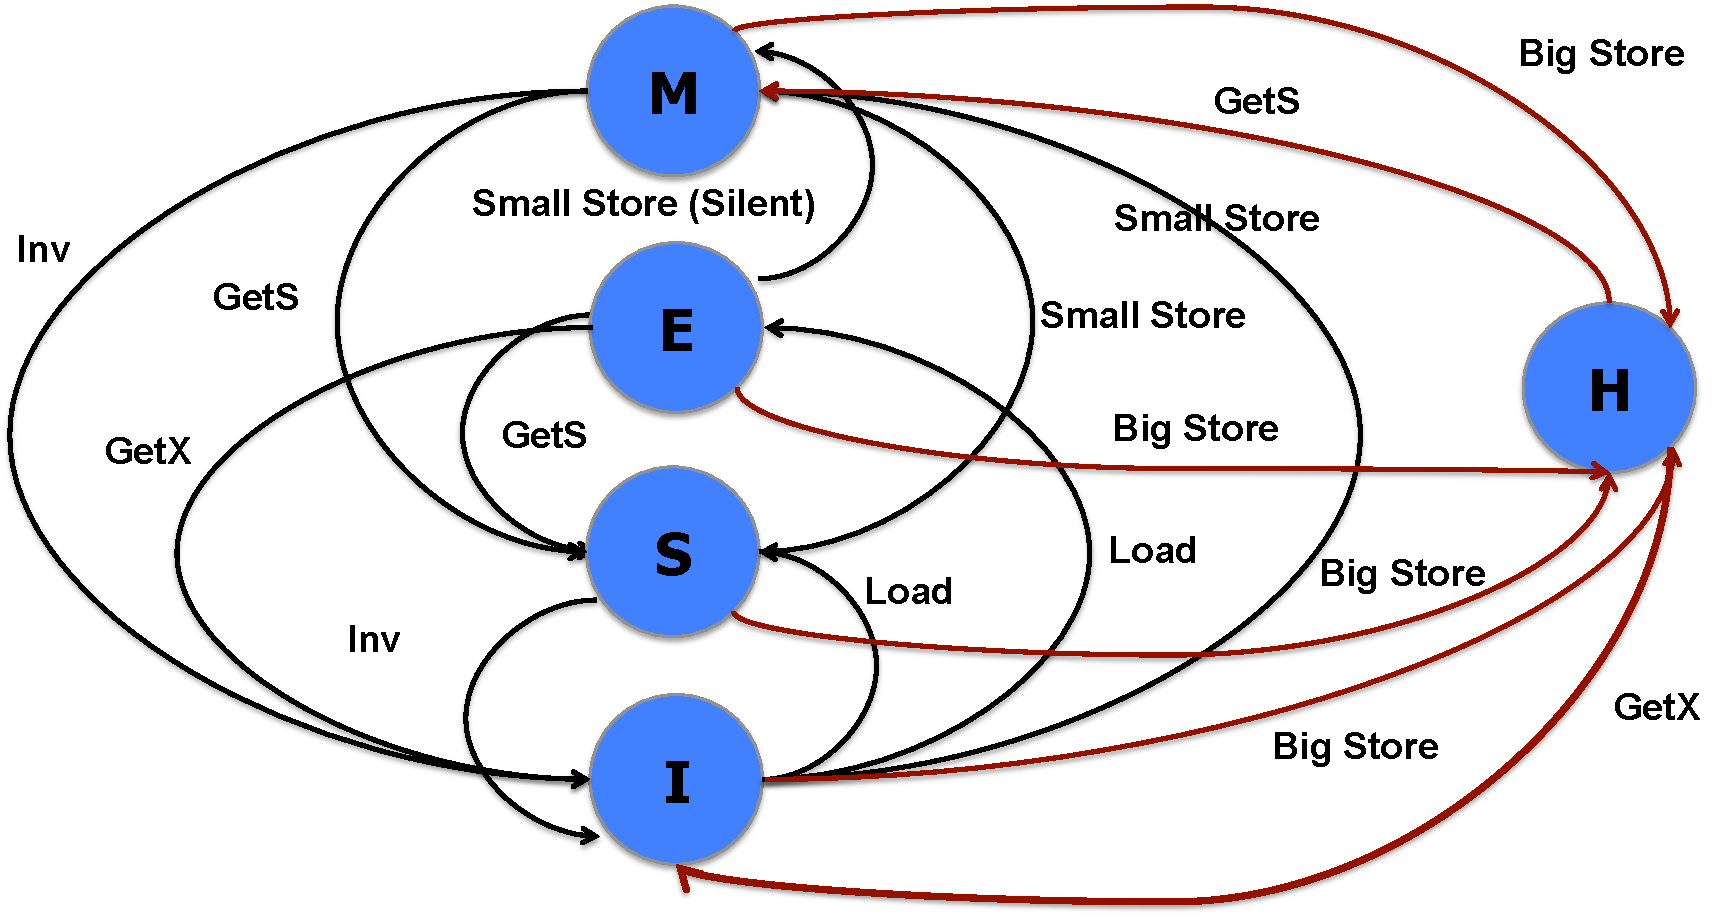
\includegraphics[height=2.5 in, width=3.2in]{figures/figure5.pdf}
  \caption{Approximate Coherence Protocol}
  \label{fig:profile}
\end{figure}

